\documentclass{scrartcl}

% Required packages
\usepackage{amsmath}
\usepackage[ngerman]{babel}
\usepackage{pdfpages}
\usepackage{enumitem}
\usepackage{nicefrac}
\usepackage{siunitx}

\setlength{\parindent}{0px}

\DeclareSIUnit\clight{\text{\ensuremath{c}}}

\begin{document}
\sisetup{per-mode=fraction}

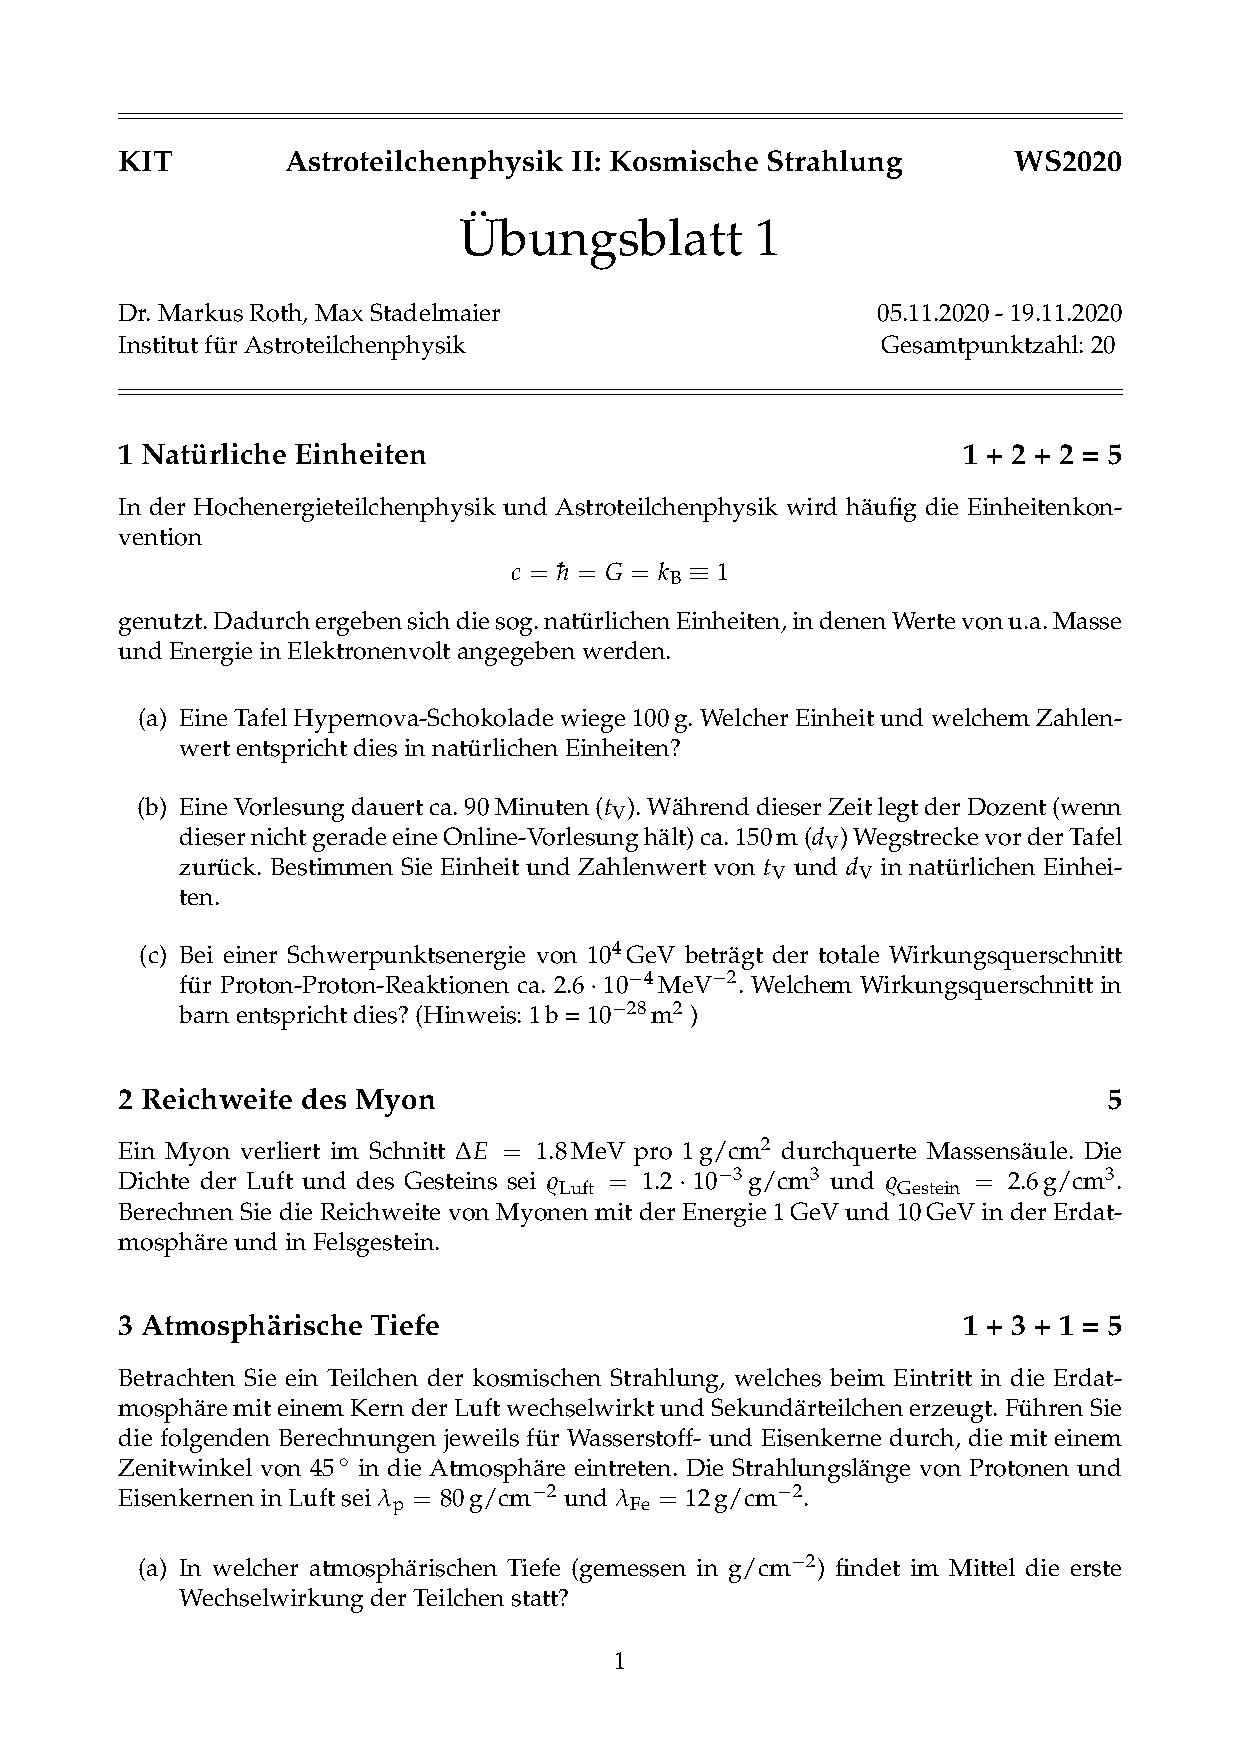
\includepdf[pages=-]{1.pdf}

\begin{center}
  \begin{huge}
    \textbf{LÖSUNGEN}
  \end{huge}
\end{center}


\section*{Aufgabe 1}

\subsection*{a)}
\SI{1}{\electronvolt\per\clight\squared} = \SI{1.783e-33}{\gram} $\Longleftrightarrow \SI{100}{\gram} = \SI{5.61e34}{\electronvolt}$

\subsection*{b)}
$\hbar = \SI{6.582e-16}{\electronvolt\second} \Rightarrow \SI{1}{\second} = \SI{1.519e15}{\per\electronvolt}$ \\
$c\hbar = \SI{197.3e-9}{\electronvolt\meter} \Rightarrow \SI{1}{\meter} = \SI{5.068e9}{\per\electronvolt}$ \\

Damit ergibt sich wie folgt: \\

$t_\text{V} = 90\cdot60\cdot\SI{1.519e15}{\per\electronvolt} = \SI{8.204e18}{\per\electronvolt}$ \\
$d_\text{V} = 150\cdot\SI{5.068e9}{\per\electronvolt} = \SI{7.602e8}{\per\electronvolt}$

\subsection*{c)}

$\SI{1}{\meter} = \SI{5.068e9}{\per\electronvolt} \Rightarrow \SI{1}{\per\mega\electronvolt\squared} = \SI{3.893e-32}{\meter\squared}$ \\
$s_{pp\rightarrow X} = \SI{2.6e-4}{\per\mega\electronvolt\squared} \cdot \SI{3.893e-32}{\mega\electronvolt\squared\meter\squared} = \SI{1.012e-26}{\meter\squared}$

\end{document}
